% This is samplepaper.tex, a sample chapter demonstrating the
% LLNCS macro package for Springer Computer Science proceedings;
% Version 2.20 of 2017/10/04
%
\documentclass[runningheads]{llncs}
%

% \usepackage{biblatex}
\RequirePackage[
  % backend=bibtex,   % Recommended is `biber`, but gives
  backend=biber,     % timeout on Overleaf
  style=numeric,   % Equivalent to elsarticle-num-names
  sorting=none,    % Adjust sorting as needed
  natbib=true      % Compatibility with natbib
]{biblatex}

\usepackage{graphicx}
% \usepackage{cite}
\usepackage{url}
\usepackage{lipsum}                     % Dummytext
\usepackage{xargs}                      % Use more than one optional parameter in a new commands
\usepackage[pdftex,dvipsnames]{xcolor}  % Coloured text etc.
\usepackage{subcaption}


% Define custom colors
\definecolor{irrelevant}{RGB}{255, 0, 0} % Red color for old text
\definecolor{old}{RGB}{128, 128, 128} % Gray color for irrelevant text
\definecolor{final}{RGB}{0, 128, 0} % Green color for final text
\definecolor{edit}{RGB}{0, 0, 255} % Blue color for notes or other text

\newcommand{\comment}[2][Comment]{\todo[inline,color=blue!20!white]{\textbf{#1}: #2}}
\newcommand{\commentside}[2][Comment]{\todo[color=blue!20!white]{\textbf{#1}: #2}}

% Increase margin text width
\setlength{\marginparwidth}{2cm}

\usepackage{scrlayer-scrpage}

% Bibliography:
\addbibresource{bibliography/phd_proposal.bib}

\addbibresource{bibliography/standards.bib}
\addbibresource{bibliography/general.bib}
\addbibresource{bibliography/intro.bib}
\addbibresource{bibliography/raspberry.bib}

\setcounter{page}{1}

% Define custom todo commands
\newcommand{\fixme}[1]{%
  \todo[color=red!20, inline, size=\footnotesize]{FIXME: #1}%
}

\newcommand{\review}[1]{%
  \todo[color=blue!10, inline, size=\footnotesize]{REVIEW: #1}%
}

% With an exclamation mark icon
\newcommand{\alert}[1]{%
  \todo[inline, color=orange!30, size=\small, bordercolor=orange!80, linecolor=orange!80]{ALERT: #1}%
}

\makeatletter
\AtBeginDocument{%
  \def\doi#1{\url{https://doi.org/#1}}}
\makeatother

\makeatletter
\renewcommand\paragraph{\@startsection{paragraph}{4}{\z@}%
                                    {2.25ex \@plus1ex \@minus.2ex}%
                                    {-1em}%
                                    {\normalfont\normalsize\bfseries}}
\makeatother

%\urlstyle{same}

%
\usepackage[colorinlistoftodos,prependcaption,textsize=tiny, disable]{todonotes}
% Used for displaying a sample figure. If possible, figure files should
% be included in EPS format.
%
% If you use the hyperref package, please uncomment the following line
% to display URLs in blue roman font according to Springer's eBook style:
% \renewcommand\UrlFont{\color{blue}\rmfamily}

\begin{document}
%
\title{
UGV Backtracking Recovery With Active Visual Landmarks Navigation:
Literature Review (Assignment)
}
%
%\titlerunning{Abbreviated paper title}
% If the paper title is too long for the running head, you can set
% an abbreviated paper title here
%

\author{Dmytro Kushnir\orcidID{0009-0006-8652-5781} }
%
\authorrunning{D. Kushnir}
% First names are abbreviated in the running head.
% If there are more than two authors, 'et al.' is used.
%
\institute{
Ukrainian Catholic University, L'viv, Sventsitskogo st. 17,  79011, Ukraine
\email{kushnir\_d@ucu.edu.ua}
}
%
\maketitle              % typeset the header of the contribution
%
\begin{abstract}
This Ph.D. research aims to enhance autonomous navigation for ground vehicles in unstructured environments using an active pan-tilt-zoom (PTZ) camera. The study investigates the application of this PTZ camera system in Unmanned Ground Vehicles (UGVs) navigation across four key aspects: (1) the impact on the accuracy and reliability of topological maps generated by improved visual landmark detection through dynamic view adjustments, (2) the robustness of visual landmark representation learning and recognition via active exploration algorithms, (3) the operational constraints and limitations of the PTZ camera, and (4) the effectiveness of navigation and path planning algorithms utilizing distant landmark recognition compared to traditional omnidirectional vision systems.

The study focuses on developing and evaluating algorithms that leverage dynamic view adjustments for improved mapping and localization. The proposed system's effectiveness will be validated through comprehensive experiments, assessing its performance against static configurations. The ultimate goal is to deliver a robust and flexible navigation solution applicable to fields such as disaster response, agriculture, and environmental monitoring.

\keywords{
Active localization \and
Outdoor navigation \and
Topological mapping \and
Unstructured environment \and
UGV \and
Point of interest \and
Visual landmarks \and
GPS-denied operation
}

\end{abstract}


\section{Introduction}

The primary focus of this Ph.D. research is to enhance autonomous navigation for ground vehicles in unstructured outdoor environments using an active pan-tilt-zoom (PTZ) camera system. The research specifically addresses the vehicle recovery problem, where a vehicle must navigate back to its starting point after losing its teleoperation signal in GPS-denied scenarios. Traditional GNSS-based navigation methods are not viable in such conditions, necessitating the use of pre-recorded data and available sensor inputs for navigation.

\paragraph{Backtracking Problem}

The backtracking problem involves guiding a vehicle back to its origin by retracing its path. This approach is particularly relevant in scenarios where a vehicle loses its control signal in unstructured environments, leading to the complete suppression of GNSS and other communication signals. In such cases, pre-recorded data from the vehicle's telemetry and sensor suite—comprising cameras, IMU, and odometry—becomes essential for navigation. While LiDAR provides precise environmental mapping and is effective for locomotion on challenging surfaces, it is often cost-prohibitive and has a limited range compared to camera systems. Consequently, this research focuses on leveraging camera-based sensory systems, which offer a versatile and cost-effective solution for visual navigation. With this setting we are dealing with classical robotics Simultaneous Localization and Mapping (SLAM) problem.

Backtracking is a subproblem within the broader scope of autonomous navigation. By solving the backtracking problem, this research will lay the groundwork for tackling more general navigation tasks in the future. The methods and technologies developed here can be extended to continuous navigation, exploration, and mission planning in complex and dynamic environments.

\paragraph{Special Features of Unstructured Outdoor Environments}

Unstructured outdoor environments are characterized by their lack of regular, predictable 3D structures, making them significantly more challenging for navigation and mapping tasks. Key features include:

    Irregular Terrain: Varying ground surfaces such as rocks, vegetation, slopes, and uneven ground pose challenges for navigation \cite{Navigation_Large_Unstructured_environments}.
    Dynamic Elements: Moving vehicles, animals, or people can unpredictably change the navigable space \cite{LocalizabilityPathPlanning}.
    Varied Vegetation: Trees, bushes, and other vegetation can obscure paths and landmarks.
    Weather Conditions: Rain, snow, and fog can affect visibility and sensor performance \cite{LocalizabilityPathPlanning}.
    Absence of Man-Made Structures: Lack of regularity and predictability of buildings, roads, and other structures complicates conventional mapping techniques \cite{LandmarksEffectivenessExperiment}.

Understanding these features is crucial for developing robust navigation and mapping systems that can operate effectively in such challenging conditions. This research aims to improve the accuracy and reliability of topological maps generated by improved visual landmark detection, enhance the robustness of visual landmark representation learning and recognition through active exploration algorithms, and investigate the operational constraints and limitations of the pan-tilt-zoom camera in comparison to traditional omnidirectional vision systems.

By addressing these challenges, the ultimate goal is to deliver a robust and flexible navigation solution applicable to fields such as disaster response, agriculture, and environmental monitoring. The advancements made in this study will not only solve the specific problem of vehicle recovery but also pave the way for more general and complex autonomous navigation tasks in the future.


\section{Related work and Research Questions}


\subsection{Visual Perception and Mapping}

% \todo[inline]{Comment: this "topic list" will not be included in the final version}
% Content by topics:
% \begin{itemize}
%     \item Visual feature extraction techniques.
%     \item Image matching algorithms.
%     \item Applications of Visual Large Language Models (VLLMs) for semantic description.
%     \item Similar works using different sensory setups.
%     \item Studies on topological mapping techniques.
%     \item Impact of accurate landmark detection on mapping.
%     \item Integration of mapping and navigation systems.
% \end{itemize}

\paragraph{Introduction to Mapping}
Mapping is a fundamental task in robotics and autonomous systems, crucial for navigation and environment understanding. The main types of mapping techniques include metric mapping, which relies on detailed geometric information, and topological mapping, which uses a network of interconnected nodes representing distinct places and the paths between them. Topological mapping is particularly attractive for its compactness and efficiency, making it suitable for environments where precise measurements are challenging to obtain \cite{HybridTopoMetricMaps}.

\paragraph{Topological Mapping}
Topological mapping represents environments using nodes and edges, facilitating tasks such as path planning and navigation. This approach is advantageous in environments segmented into distinct, recognizable areas. Unlike metric maps, which require detailed geometric information, topological maps rely on the relative positions of nodes, making them efficient for spatial representation. However, the challenge arises in more complex environments where place recognition becomes unreliable due to the lack of metric information. This limitation can cause significant issues in large unstructured environments, as the robot may struggle to distinguish between similar-looking areas, breaking the logic of the topological map and hindering reliable navigation.

\paragraph{Hybrid Mapping Approaches}
Simon and Dudek have proposed a hybrid approach combining topological and metric maps to address the challenges of navigation in large, unstructured environments. This method utilizes local metric maps (islands of reliability) connected topologically to mitigate accumulated errors over large spaces. Simhon and Dudek's work organizes local maps in a topological structure to maintain accuracy while avoiding large-scale error accumulation \cite{HybridTopoMetricMaps}. This approach aligns with our goal of developing robust navigation systems for UGVs in unstructured outdoor environments by leveraging visual landmarks for improved place recognition and localization.

\paragraph{Place Recognition}
The concept of place recognition is integral to autonomous navigation, ensuring reliable localization and mapping. Traditional methods of place recognition often depend on distinct and consistent landmarks, which may not always be present in unstructured or dynamic environments. The paper "Placeless Place-Recognition" by Lynen et al. \cite{PlacePlaceRecognition} addresses this challenge by introducing an innovative approach that relies on unique environmental characteristics rather than distinct landmarks. This method leverages advanced feature extraction techniques and a probabilistic framework to create a robust representation of places, invariant to changes in viewpoint, lighting, and environmental conditions. By focusing on the probabilistic matching of these features, the system enhances the reliability of place recognition even in challenging and unstructured environments.

The \textit{placeless} place recognition approach is particularly relevant for our research, which aims to improve the accuracy and reliability of topological maps generated by UGVs in unstructured environments. The feature-based matching and probabilistic models proposed by Lynen et al. can be integrated into our visual landmark detection and recognition systems, providing a robust solution for navigating environments with irregular terrain, dynamic elements, and varying vegetation. Integration of this approach with pan-tilt-zoom cameras will be investigated in the context of Research Questions 1 and 2 by enhancing the robustness and accuracy of our topological mapping framework, ensuring reliable UGV navigation and mapping in diverse and challenging outdoor settings.

\paragraph{Indoor vs. Outdoor Visual Localization}
Given our specific application domain and challenges, we focus on outdoor applications. However, the advancement of visual localization algorithms has primarily taken place within the context of indoor (laboratory) applications. Consequently, we are also exploring these indoor algorithms for their potential applicability to our work \cite{IndoorsSparseLandmarks, LandmarksEffectivenessExperiment}.

Indoor environments lack GPS but provide optimal conditions for camera-based visual registration. Therefore, research in this field has methodological value for us. Well-established techniques for visual navigation have emerged \cite{LandmarkGraphBasedIndoorLoc}, along with numerous robust methods for agent self-localization. These approaches are currently being adapted to large-scale outdoor navigation.

\paragraph{Visual Landmarks in UAV and UGV Navigation}
Typically, the UAV visual navigation task is framed at altitude with a downward-facing camera setup, but there are subfields where the settings are very similar to those of UGVs. An example is research on low-altitude navigation in urban environments by Liu \cite{POI_and_store_signature}, where the approach was developed for low-altitude UAVs based on visual landmarks. Notably, the urban environment they addressed is highly structured and rich in strong visual localization features. The author highlighted this environment property by utilizing text-based Points of Interest (POIs), incorporating textual signatures visible on streets. Such an urban or suburban setup can serve as an intermediate step toward the application of open, unstructured environments by providing a robust framework for visual-based localization. Also, this is especially interesting work since it also gives a hand to the VLLMs-based description-based navigation.

\paragraph{Limitations of Mapping Types for Large-Scale Unstructured Navigation}
Our map surveying approach from the first stage involves two key aspects: reliable positioning relative to our "visual landmarks" and the localizability of local environments, as elaborated in \cite{LocalizabilityPathPlanning}. This dual focus is essential for ensuring safe graph traversal. Furthermore, we intend to leverage established techniques to seamlessly incorporate existing solutions, particularly when addressing the challenges posed by battery life constraints in the context of the backtracking problem.

Localization based on visual landmarks is a well-established classic problem \cite{LandmarksFoundation} that showed its effectiveness \cite{LandmarksEffectivenessExperiment} and became the classic approach. This method is an auxiliary navigation tool in ambiguous environments, where metric maps are typically constructed using specialized measurement tools like LIDAR and range measurement sensors. Although these maps accurately represent the environment, they struggle in cases with repetitive obstacle shapes, leading to reduced reliability. To overcome this, introducing a reliable visual signal source can resolve ambiguity, as highlighted in \cite{LandmarksEffectivenessExperiment}. Our approach employs visual landmarks as beacons for consistent and dependable localization, and the best approach for their selection and representation using the active pan-tilt-zoom camera is one of the research questions that we plan to leverage in the course of our work.

In the context of navigation and mapping in large unstructured environments, the classification and utilization of visual landmarks play a crucial role. The work on Hybrid Metric-Topological Maps (HYMM) emphasizes storing Occupancy Grid (OG) maps for later information retrieval and evaluating which high-level features of the landscape can be considered landmarks. This approach typically operates in offline mode, which may not be feasible in dynamic settings. Furthermore, it relies on OG maps generated by LIDAR or RGB-D cameras, presenting a challenge when using purely visual mapping techniques due to the sparse information available. For effective feature selection, an active survey of potential landscape objects is required, which is impractical at the initial mapping stage. This highlights the need for real-time, robust landmark detection mechanisms that can operate effectively in unstructured environments \cite{Navigation_Large_Unstructured_environments}.


\begin{figure}
    \centering
    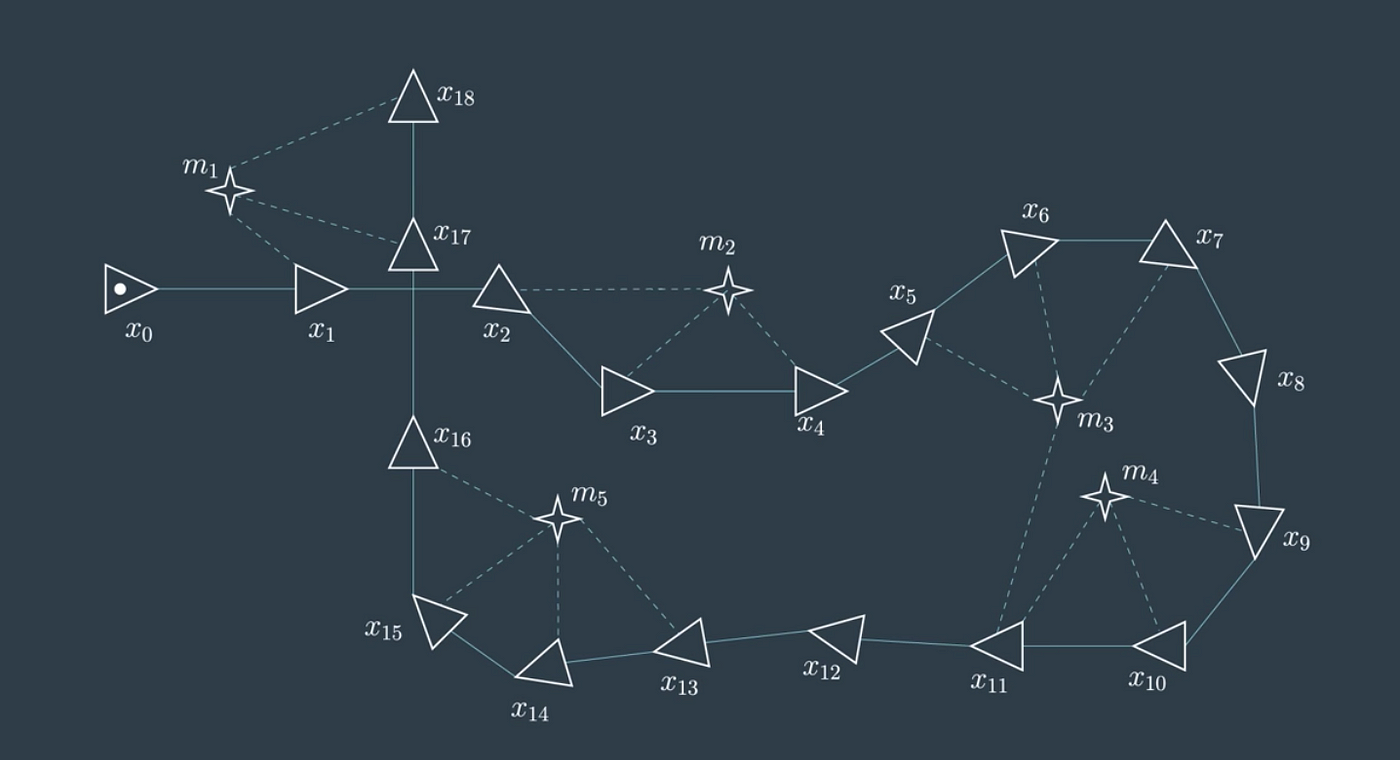
\includegraphics[width=0.8\linewidth]{img/pose-landmark-graph.png}
    \caption{Map in the form of a navigation graph. Triangle: robot poses during the mapping process, also graph nodes that are recognized as "Places."
    Stars: visual point of interest: landmarks. Dashed line: observation. Solid line: movement record. }
    \label{fig:pose-landmark-graph}
\end{figure}

While Visual Large Language Models (VLLMs) offer an intriguing solution within topological mapping frameworks, their application in large-scale unstructured environments still requires significant advancements. VLLMs excel in indoor navigation scenarios where controlled environments allow for consistent visual feature extraction and recognition. However, in outdoor settings, the stability of visual representations and their recognition from various viewpoints and distances remains a challenge. The work on semantic mapping further underscores the limitations of current technologies, necessitating robust methods to ensure consistent landmark recognition despite changes in perspective and environmental conditions \cite{RangeSensorsEvalutation}. Addressing these challenges involves not only improving visual feature extraction techniques but also integrating these advancements into a cohesive system capable of real-time operation in dynamic, unstructured environments.

\subsection{Research gap: Visual Large Language Models navigation in environments of different semantic density}

\comment{@To Maks.Davydov: I don't know where is the proper place to put those 'Research gap' materials. It feels like those has to be placed inside relevant research block as we identify it, but the proposed research plan fits to the Objective and Methodology part.}

While Visuals Large Language Models (VLLMs) offer an intriguing combination with topological mapping frameworks, their application in large-scale unstructured environments still requires significant advancements. VLLMs excel in indoor navigation scenarios where controlled environments allow for consistent visual feature extraction and recognition. However, in outdoor settings, the stability of visual representations and their recognition from various viewpoints and distances remains challenging. As the current rate of publications in the semantic navigation field proposes here, the advancements in semantic mapping may further impose questions on the importance of dedicated visual navigation frameworks. Addressing these questions, we will also improve visual feature extraction techniques and integrate these advancements into our system.
Such work could be performed in the context of continuing the current research line on the indoor navigation of embodied AI agents done by the robotics researchers \cite{PointGoalNavUCU} and ongoing research avenue aimed at research of the scene descriptions provided by VLLMs.

\textbf{The hypothesis basis for this research gap:}
VLLMs can perform visual navigation tasks only in environments filled with semantically rich visual information, such as usual home environments. They will still perform moderately in semi-structured outdoor environments filled with human-made objects that can be described and uniquely identified by description: we have such environments in urban landscapes. The worst performance VLLMs will show in unstructured outdoor environments is in wild landscapes with sparse objects that can serve as description-based localization.
We can reuse the same topological mapping frameworks for the mapping and localization of UGV as in the main vision-based experiment track. This research will show the limitations of the popular now-based navigation and explain why the proposed research aims are important and will preserve its importance in the future.
Also, we will get useful insight from investigating the attention model of the VLLMs. The hypothesis here is that objects that are good as landmarks with their semantic description are, at the same time, good visual landmarks for vision-based navigation. We can also check this hypothesis during proposed experiments.


\comment{Fine to read}
\subsection{Operational Constraints in Autonomous Navigation System}

\comment{Considering splitting this subsection into two parts. A review of resources for Q3 and Q4 ends up being not very dependent.}

\begin{itemize}
    \item Analysis of operational constraints in UGV systems.
    \item Comparative studies of different camera setups.
    \item Research on utility-based exploration, active localization.
    \item Visual-constrained path planning methods.
    \item Path planning within topological maps.
\end{itemize}


\paragraph{Challenges in Unstructured Outdoor Environments}

Unstructured outdoor environments present significant challenges for autonomous navigation systems. The lack of regular, predictable 3D structures makes navigation and mapping particularly difficult. These environments often suffer from irregular terrain, dynamic elements such as moving vehicles or animals, varied vegetation that can obscure paths, changing weather conditions, and the absence of man-made structures. Without GNSS, maintaining reliable localization becomes exceptionally challenging, even for tasks as fundamental as backtracking. Understanding these features is crucial for developing robust systems capable of effective operation in such demanding conditions.

\paragraph{Visual Navigation Using PTZ Cameras}

PTZ (Pan-Tilt-Zoom) cameras are more commonly employed in UAV navigation systems than in UGV systems. This is largely due to the weight limitations and the need for versatile functionality in UAVs, where a single PTZ camera can serve multiple purposes. The ability to zoom is particularly essential for UAVs to provide detailed views from high altitudes. Additionally, the pan and tilt functions support tracking and object detection, which are critical in dynamic environments. However, the pan-tilt functionality is rarely utilized for navigation purposes.
UAV Navigation with PTZ Cameras

In UAVs, PTZ cameras enhance visual localization and navigation in GPS-denied environments. Research by Patel et al. \cite{PointMeIntoRightDirection} demonstrates the benefits of using a gimballed stereo camera for localization, showing improved performance and robustness by actively controlling the camera’s viewpoint during flight. This setup allows the UAV to maintain localization even under varying velocities and environmental conditions by minimizing viewpoint orientation errors and pointing the camera's optical axis at previously observed landmarks.

Another study by Skjong et al. \cite{SearchAndTrackingGimbal} explores the use of visual teach and repeat (VT\&R) techniques for UAVs, employing a gimballed camera to ensure reliable navigation in scenarios where GPS is unavailable. The research highlights the effectiveness of using gimballed cameras to compensate for the UAV's dynamic movements, thus maintaining a stable viewpoint and improving the robustness of visual localization.


\paragraph{UGV Navigation with Omnidirectional and Rotating Cameras}

In contrast, UGVs typically utilize omnidirectional cameras, such as catadioptric or fisheye cameras, which provide a 360-degree view. These setups offer simpler operational logic compared to PTZ cameras. For instance, multicamera systems or rotating cameras can be used to create panoramic images, which are crucial for comprehensive environmental awareness and navigation. However, these configurations lack the zoom functionality, limiting their ability to perform long-range visual navigation.

A relevant study in this context is by Peleg et al. \cite{Omnistereo_Shmuel}, which discusses the usage of omnistereo vision for robot navigation. The research illustrates how panoramic stereo images can be generated using multiple cameras or rotating setups to achieve a wide field of view necessary for navigation in unstructured environments.
Identified Research Needs

Overall, we can identify several research gaps that are crucial for the effective PTZ camera application in our context:

\begin{itemize}

    \item \textbf{Integration of Zoom Functionality in UGVs:}
    UGV navigation systems typically lack the ability to perform long-range visual navigation due to the absence of zoom functionality. Integrating PTZ cameras into UGV systems could bridge this gap by providing both wide-area coverage and detailed views of distant objects, thereby enhancing situational awareness and navigation capabilities.

    \item \textbf{Complexity of Pan-Tilt Operations:}
    While PTZ cameras offer versatile functionality, the complexity of pan-tilt operations poses a challenge. Research needs to focus on developing robust algorithms that can effectively utilize the pan-tilt functions for navigation without overwhelming the system’s computational resources.

\end{itemize}

By addressing these gaps, future research can enhance the reliability and robustness of visual navigation systems using PTZ cameras, contributing significantly to the advancement of autonomous
navigation technologies.

\paragraph{Active Localization and Path Planning under Localizability Constraints}

The integration of PTZ cameras into UGVs offers a unique opportunity to enhance active localization. Unlike static or limited mobility cameras, PTZ cameras can adjust their viewpoint to focus on specific landmarks or areas of interest, thereby improving localization accuracy. This capability allows robots to perform long-range visual navigation, going beyond precise road backtracking and enabling them to re-localize themselves by actively moving around and utilizing the PTZ camera to scan the environment for recognizable features.

Active localization has become a well-established research area with diverse approaches. The seminal work by Burgard et al. introduced active mobile robot localization, highlighting the need for robots to control their movements to optimize localization \cite{burgard1997active}. This research area has evolved significantly, with various problem setups and approaches being explored \cite{BurgardActiveMarkovLocaliation, AutonomousRoboticExplorationGraph}. Our goal is to evaluate multiple concepts to determine the most effective one for our specific application.

\paragraph{Path Planning under Localizability Constraints}
Path planning under localizability constraints has been explored in depth in the literature. Our approach involves reliable positioning relative to our "visual beacon" and the localizability of local environments, as elaborated by Liu et al. \cite{LocalizabilityPathPlanning}. This dual focus is essential for ensuring safe graph traversal. Furthermore, we intend to leverage established techniques to seamlessly incorporate existing solutions, particularly addressing challenges posed by battery life constraints in the context of the backtracking problem.

\textit{The hybrid topological-metric maps approach}, where local metric maps (islands of reliability) are connected topologically, provides a robust solution for large-scale navigation by mitigating error accumulation \cite{HybridTopoMetricMaps}. This concept is particularly relevant for UGVs operating in unstructured environments, as it allows for efficient route planning and reliable navigation using a combination of metric and topological data.

\paragraph{Localization ambiguity}:
The assessment of localization ambiguity should draw from both: the overall environmental information and operation field-specific data gathered during the POI mapping. Researchers often devise their own "localization ambiguity" criteria tailored to their problem context \cite{AmbiguityGridMap} \cite{LandmarksEffectivenessExperiment}.

\paragraph{Informative Path Planning}
Active mapping and path planning under localization uncertainty are critical aspects of autonomous navigation in unstructured environments. Popović et al. \cite{InformativePathPlannin_under_uncertainty} introduced an informative planning framework for active mapping that explicitly accounts for pose uncertainty in both mapping and planning tasks. Their strategy uses a Gaussian Process (GP) model to capture environmental fields, coupled with a utility function that integrates localization and field mapping objectives. This approach has shown to significantly reduce pose uncertainty and map error, making it highly relevant for our research on improving the robustness and accuracy of navigation systems in complex environments.

\subsubsection{Research Goals for Informed Navigation and Planning Policies}

The culmination of our research efforts aims to integrate the aforementioned approaches into a cohesive system that ensures optimal exploration and reliable navigation. This involves developing planning algorithms that are not only informed by the current state of the environment but also adapt to changing conditions in real-time. Such algorithms should be able to leverage the active localization capabilities provided by PTZ cameras, thus enabling robots to dynamically adjust their paths based on the quality and reliability of the information available.

Future research in improved path planning with PTZ camera enhanced capabilities should focus on:

\begin{itemize}
    \item \textbf{Utility-Based Exploration:}
    Developing exploration strategies that balance the trade-offs between exploration and exploitation, ensuring that robots can efficiently gather information about their environment while maintaining robust localization.

    \item \textbf{Adaptive Planning Policies:}
    Creating planning policies that can dynamically adapt to the environment, taking into account the uncertainty in localization and the availability of visual landmarks.

    \item \textbf{Enhanced Visual Processing:}
    Advancing visual processing techniques to better utilize PTZ cameras for detailed environment analysis, including long-range detection and recognition of landmarks.

\end{itemize}

We aim to push the boundaries of current autonomous navigation systems by addressing these research goals, making them more reliable and efficient in real-world applications. This comprehensive approach will bridge the existing research gaps and pave the way for advanced navigation systems capable of reliable operations in the most challenging environments.

\subsection{RQ1: Visual Landmark Detection and Recognition}

\comment{Reason why placed here: This question addresses the core technology and its enhancement—improving landmark detection and recognition—which is fundamental to the other questions.}

% \todo[inline]{Fill up Add on visual feature extraction, image matching, and application of the VLLMs for semantics description. Similar work on another sensory setup. }

\subsubsection{Research question:}
    How does the active exploration algorithm based on a pan-tilt-zoom camera with stabilization improve the robustness of visual landmark representation learning and recognition?

\subsection{RQ2: Topological Mapping Accuracy}

\comment{Reason why placed here: Building on the improved detection and recognition capabilities, this question explores how these enhancements impact mapping accuracy, a crucial navigation aspect.}

\subsubsection{Research question}
    How does the improved accuracy and robustness of visual landmark detection, achieved through the use of an active pan-tilt-zoom camera, affect the accuracy and reliability of topological maps generated by the UGV in various unstructured environments?

\subsection{RQ3: Operational Constraints}

\comment{Reason why placed in this order: After understanding the core technology and its impact on mapping, it's important to identify the practical limitations and operational constraints and how this solution compares to existing alternatives.}

\subsubsection{Research Questions:}
    What are the operational constraints and limitations of using a pan-tilt-zoom camera for visual landmark-based navigation in unstructured environments?
    How does it exceed alternative solutions?

    % \todo[inline]{
    % The particular focus for the proposed research attacking the outlined research questions is ...
    % }

\subsection{RQ4: Navigation and Path Planning}

\comment{Reason why placed in this order: This question focuses on the practical application and effectiveness of the technology in real-world navigation and path planning, leveraging the previously discussed improvements and constraints.}

% \todo[inline]{Add materials on utility-based exploration, on visual-constrained path planning}
% \todo[inline]{IMPORTANT!: make explanation about path planning in TopologicalMaps}

\subsubsection{Research question:}
    How can algorithms that utilize the ability to recognize and determine the distance to distant landmarks with a pan-tilt-zoom camera improve the navigation and path planning effectiveness of Unmanned Ground Vehicles (UGVs) in returning to their home base compared to traditional omnidirectional vision systems?

\section{ Background, Objective, and Methodology }

\subsection{ The Background for the Proposed Research }

% \begin{itemize}
% \item \todo[inline]{What SoTA will be used as the background for the solution? }
% \item \todo[inline]{Compare with Husky navigation stack}
% \item \todo[inline]{- Including your results in the Y1 of the Program}
% \item \todo[inline]{Why are these background components chosen (based on Literature review)?}
% \end{itemize}



\paragraph{ROS technological stack} For the development of the solution, we are planning to use The Robot Operating System (ROS/ROS2) \cite{ROS2}.  ROS is an open-source middleware framework that provides a structured communication layer above the host operating systems of a heterogeneous computer cluster. It is widely used in robotics research and development due to its robust ecosystem and extensive library of tools and packages. ROS enables the seamless integration of sensors, actuators, and algorithms, facilitating the simulation-to-real transition. This capability is crucial for our project as it allows us to validate our navigation algorithms in a simulated environment before deploying them in real-world scenarios. The selection of platform, sensors, and baseline solution depends on those elements' ROS compatibility.

\paragraph{Navigation modules} In addition to its support for simulation, ROS offers a modular architecture that enhances the flexibility and scalability of robotic systems. This modularity allows for the separation of different functionalities into distinct, reusable components. For example, in our navigation stack \ref{fig:ROS-navigation}, obstacle avoidance, and long-range path planning are treated as separate entities. The obstacle avoidance module operates at a lower level, reacting to immediate hazards and ensuring the robot's safety in real-time. In contrast, the long-range planning module focuses on high-level route planning, using topological maps and landmark-based navigation to guide the robot over extended distances. This hierarchical approach ensures that each module can be developed, tested, and optimized independently, leading to a more robust and efficient overall system. By utilizing ROS's modular framework, we can easily integrate new sensors and algorithms, adapt to different operational requirements, and achieve a high degree of interoperability between various system components, making comparative experiments of different system compositions possible.

\begin{figure}
    \centering
    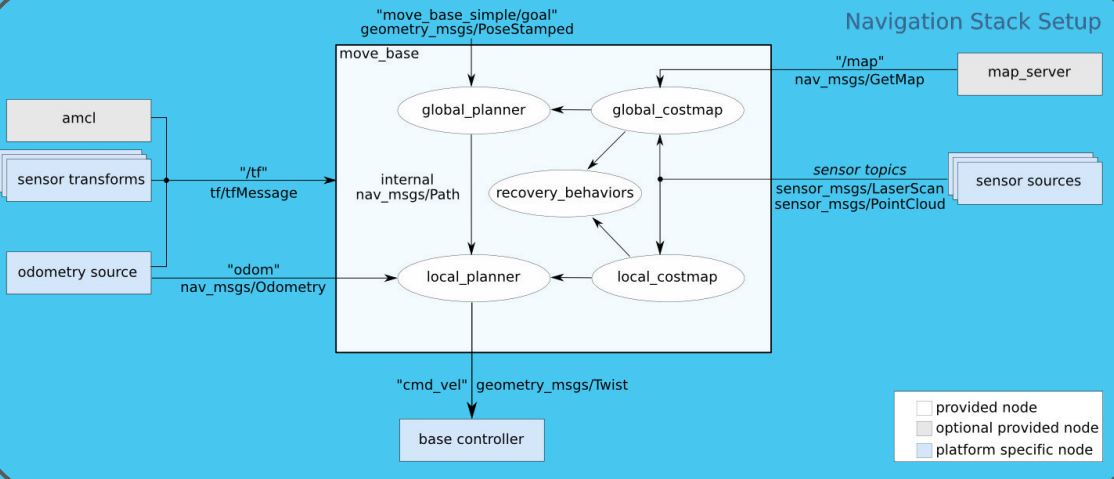
\includegraphics[width=0.75\linewidth]{img/ROS_navigation.png}
    \caption{Structure of the ROS navigation infrastructure}
    \label{fig:ROS-navigation}
\end{figure}

\paragraph{Integration}
We will commence with miniature experiments within campus facilities, focusing on an indoor setup for preliminary validation of intermediate results and pipeline performance. Given the distinct nature of visual landmarks mapping, this approach will be more effective for actively traversing the visual landmarks graph map.
Field testing will be essential during the course of our research. Thus, we must develop a ROS software package that is responsible for long-term navigation and is seamlessly integrated into our platforms. This package will facilitate interaction with video streams and telemetry data as inputs while receiving movement direction commands as outputs for backtracking. The only other component will be the creation of a ROS wrapper for our PTZ camera. Due to our progress on the Y1 in work with this equipment, this will be a more technical solution rather than a high-risk endeavor.

\paragraph{Visual Teach and Repeat (VT\&R) as the Baseline Framework}

For our research, we selected the Visual Teach and Repeat (VT\&R) framework, which is widely used for visual navigation. VT\&R fits our problem setup due to its emphasis on route replication. For backtracking tasks, the teach phase allows the robot to familiarize itself with the route under controlled conditions. During the recovery phase, the robot can navigate back to its starting point using pre-recorded data, ensuring reliable navigation even in complex environments. VT\&R is supported by ROS (Robot Operating System) packages, facilitating integration and allowing us to enhance the framework with different camera configurations, including PTZ cameras. We will compare PTZ cameras with omnidirectional and simple perspective cameras to determine the optimal setup. This analysis will highlight the strengths and limitations of each configuration, ensuring a fair assessment of VT\&R's performance in different environments.

Warren et al. \cite{PointMeIntoRightDirection} demonstrated that using a gimballed camera on UAV in VT\&R enhances visual localization by allowing active viewpoint manipulation, significantly improving localization accuracy and robustness, providing a solid foundation for our research questions.


\comment{This one is ready to read}

\subsection{Informal Problem Setup Conditioning}

\paragraph{GPS-Denied Unstructured Environment}:
The operational conditions include a total denial of GPS signal; the proposed approach cannot rely on GNSS during either the mapping or the backtracking phase. We decided to avoid actual metric mapping and precise localization in the operational environment. Visual landmarks navigation graphs should be used for long-range navigation to traverse back to the home base node. Graph nodes will contain all required additional data about the landmarks and their neighboring nodes. The nodes will be split into two categories: \textbf{Places} -- locations that the robots have visited that are visually distinguishable based on observations \cite{PlacePlaceRecognition}, and \textbf{Landmarks} -- individually recognizable objects in the environment used for determining information about Places.

\paragraph{Mapping Constraints}:
Since we are working on a platform recovery scenario for a system that lacks true autonomy for mission planning and execution, the problem setting and restrictions are similar to those described by Warren in the "No Place Like Home" research \cite{warren-ral19-no-place-like-Home}. According to this formulation, during the \textbf{learning} phase, the system operates under the control of the operator, and full active exploration autonomy is infeasible under such constraints. Therefore, the value of the independent pan-tilt-zoom camera increases; it can independently explore the observable environment and map visual beacons.

In the \textbf{returning} home phase, there are no stringent operational time restrictions, but there are natural constraints related to the remaining battery charge that serve as critical limitations.

\paragraph{Problem Relaxation Opportunities}:
There are many scenarios when we have an opportunity for repeated observations of the same territory. These are typical in agricultural settings when a UGV travels back and forth between the operation field and the base station, patrolling routes, or when smart platforms are used for transportation purposes. Additionally, we can simplify the task by focusing on cases where time constraints are not crucial, such as during the mapping phase of automated search and rescue missions. In this setup, we could consider an active approach for landmark position refinement during the mapping phase.

\paragraph{Expected Restrictions}:
Routes have to be performed in regions with a limited number of distinctive landmark features, such as uniform vegetation regions or fields. This is motivated by the fact that feature-rich locations may be restricted for operation due to safety conditions or specific setups, such as ecological, forestry, or agricultural applications.

\paragraph{Envisioned Problem Attack Direction}:
We plan to address localization ambiguity in outdoor unstructured environments where visual beacons are sparse or distant from the actual operational route. Our hypothesis is that with the PTZ camera, the UGV system can exploit zoom and positioning capabilities to use distant, uniquely identifiable landmarks to overcome the limitations of large-scale outdoor unstructured environments.

\subsection{Approaching the Goal}

To begin, we need to establish a stable testing environment for comparison with a baseline method \cite{VisualTeachAndRepeat}. This entails designing performance metrics, which we envision as the percentage of successful UGV recoveries to the home base.

\paragraph{Success Evaluation}
As we are focusing on the lost UGV recovery scenario, there are no stringent real-time reasoning and execution speed requirements. The main performance criterion is platform safety and the chances of success, measured by the \textbf{Percentage of Successful Recoveries to the Home Base}, where success is defined as the distance being less than a threshold to the home base coordinate point. This criterion can only be measured through repeated trials with randomized episode settings or environment configurations.

\paragraph{Secondary Performance Measurements}
These measurements will rank the performance of tested solutions that have the same performance regarding the basic success criteria.
\begin{enumerate}
    \item Distance to the home base at the end of the episode (if the objective is not achieved).
    \item Accumulated error of closest distances to the planned route (in strict return home by route scenario).
    \item Distance traveled.
    \item Time spent on the episode.
    \item Energy usage.
    \item Other relevant metrics.
\end{enumerate}

\subsubsection{Visual Landmark Detection and Recognition}

The approach for selecting and learning visual landmarks representation can be developed and tested independently from the rest of the pipeline and without the UGV platform. This goal targets Q1 in isolation. Here, we can conduct many individual experiments with generated object views from different orientations taken from outdoor object datasets like Paris-Carla-3D \cite{ParisCarla3D}.

\begin{enumerate}
    \item Develop a standalone landmark representation and matching system.
    \item Evaluate landmark recognition in a simulated environment with varying object positions and lighting conditions.
    \item Transfer the problem to a realistic simulated environment, including distance to landmark estimation.
    \item Implement recognition of several landmarks and triangulation.
    \item Develop landmark selection where regions of interest in the image are not known.
    \item Change the setting to a PTZ camera on a moving vehicle, allowing offline processing.
    \item Conduct experiments in a real-world setup.
    \item Enforce online processing.
    \item Integrate learning and active localization with path planning for the UGV.
\end{enumerate}

\subsubsection{Topological Mapping Accuracy and Operational Constraints}

This research question is tightly coupled with the detection of visual landmarks. To partially decouple them, we can start experiments using artificial landmarks like ArUco markers \cite{sampathkrishna2022aruco} that can be placed in both real and simulated environments. The goal is to investigate performance improvements with PTZ cameras.

\paragraph{Visual sensors} We will compare the following setups:
\begin{enumerate}
    \item Static forward-facing cameras.
    \item Forward and backward-facing cameras for simple backtracking guided by pre-recorded video during the learning phase.
    \item Panoramic view created by image stitching with PTZ cameras.
    \item Genuine 360-degree cameras.
    \item PTZ cameras.
\end{enumerate}

\paragraph{Environment complexity} Environments will include simulations and real-world experiments at different stages:
\begin{enumerate}
    \item Basic trials with artificial markers.
    \item Indoor environment mapping.
    \item Outdoor semi-structured urban landscapes.
    \item Outdoor unstructured environments like parks and natural landscapes.
\end{enumerate}

\paragraph{Landmarks locations} We will investigate the location and distribution of landmarks, addressing Q3 about operational constraints:
\begin{enumerate}
    \item Landmarks as waypoints on the route.
    \item Landmarks offset from the route.
    \item Scattered landmarks with varying distributions close to the route.
    \item Scattered distant landmarks requiring zoom for accurate localization.
\end{enumerate}

Operational constraints will also be investigated and reported qualitatively regarding real-world factors such as surface types, vegetation height, lighting conditions, and specific natural environments like forests, grasslands, and mountains.

\subsubsection{Navigation and Path Planning}

The main goal is to determine whether active exploration outperforms passive observation policies in vehicle recovery scenarios and the impact of PTZ cameras in this context.

We will evaluate the reliability of the navigation system with different path-planning approaches. This is a later phase of research since it relies heavily on a functioning navigation pipeline. Advanced path planning approaches will highlight the extent of operational constraints and benefits of PTZ cameras through their additional degrees of freedom.

The main avenues of these experiments are:
\begin{itemize}
    \item Active localization and environment exploration \cite{BurgardActiveMarkovLocaliation, AutonomousRoboticExplorationGraph}.
    \item Path planning with localizability constraints \cite{LocalizabilityPathPlanning, HybridTopoMetricMaps}.
    \item Informative path planning under uncertainty \cite{InformativePathPlannin_under_uncertainty}.
\end{itemize}



% \todo[inline]{What methodology will be used to guide the research process toward the foreground?}

% \todo[inline]{
% \begin{itemize}
%     \item - Exploratory research;
%     \item - Methodology refinement, if any
%     \item - Framework / architecture / model / dataset development
%     \item - Experimentation
%     \item Why this methodology?
%     \item To whom will the results be compared (cross-evaluation)?
% \end{itemize}
% }

\comment{Fine to read}

\section{Resources}

% \todo[inline]{
% \begin{itemize}
%     \item What are the required and available resources for the proposed research, including dataset(s)?
%     \item Why these?
%     \item What of these are developed / will be developed in the proposed research project?
% \end{itemize}
% }

\subsection{Platform}
\subsubsection{Husky Unmanned Ground Vehicle (UGV) by Clearpath Robotics}

The Husky UGV \cite{clearpath_husky_ugv} is a robust, outdoor-ready platform widely used in research for prototyping and autonomous robotics. It has a moderate size that allows for usage of the platform in both indoor and outdoor operations \ref{fig:Clearpath Husky size specs}. It supports a variety of payloads, including stereo cameras, LIDAR, GPS, and IMUs. The Husky’s integration with ROS (Robot Operating System) makes it an excellent choice for developing and testing navigation algorithms.

\begin{figure}
    \centering
    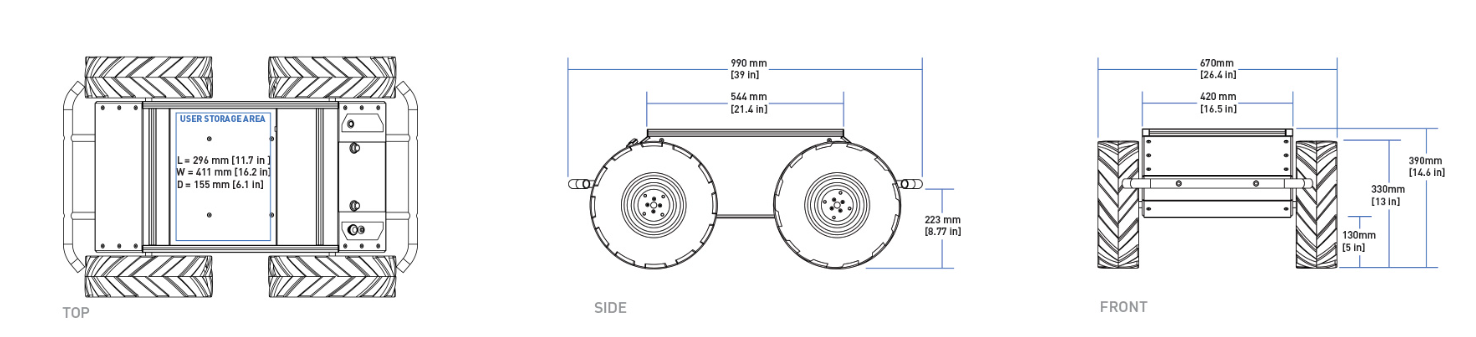
\includegraphics[width=1\linewidth]{img/HuskyScheme.png}
    \caption{Clearpath Husky UGV size specification}
    \label{fig:Clearpath Husky size specs}
\end{figure}

\textbf{Platform Equipment:}

For reliable long-range operations in outdoor environments, we will utilize the Husky platform as the basis for our sensory setup, comprising several critical components: LIDAR and RTK GPS. Similar kinds of sensors with very close characteristics have been successfully used on the Husky UGV platform for precision-critical tasks, such as infrastructure inspection \cite{AutomatedBridgeInspection_UGV_2019}, supporting the precision characteristics of our proposed setup. The visual appearance of such configuration is depicted on \ref{fig:Husky equipped}.

\begin{figure}
    \centering
    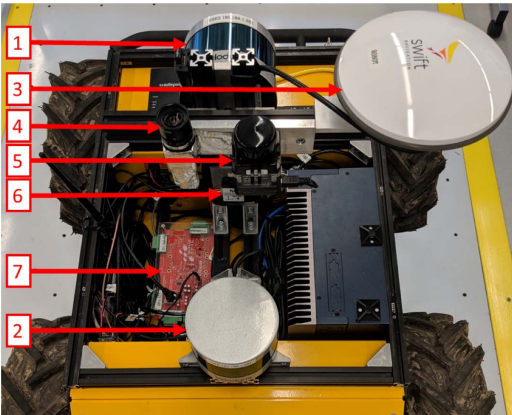
\includegraphics[width=0.75\linewidth]{img/Husky_with_equipment.png}
    \caption{Details of the sensors mounted on the UGV, labeled sensors: (1) vertical lidar (not required in our setup), (2) horizontal lidar, (3) GPS antenna, (4) vision camera, (5) IR camera (optional in our setup), (6) IMU, and (7) trigger board. Image from \cite{AutomatedBridgeInspection_UGV_2019}}
    \label{fig:Husky equipped}
\end{figure}


\subsubsection{External navigation system}
To measure localization accuracy during outdoor experiments, we need some sources of reliable positioning data that could be treated as ground truth. High precision is required to use it for the reliable comparison of different approaches and for the results to be acknowledged. Such a source has to be independent of any sensory system used for our platform localization, so we need a standalone solution for this purpose. One of the few reliable platforms with available ROS integration on the market and the  Vision RTK2 kit from the Fixposition \cite{fixposition_vision_rtk2} with capabilities of high precision GNSS positioning, IMU, and visual odometry that are fused together. Visual appearance of this kit setup is depicted on \ref{fig:Fixposition RTK-2 kit}. This device will also serve as the source for position data in the datasets we plan to collect for offline processing.

\begin{figure}
    \centering
    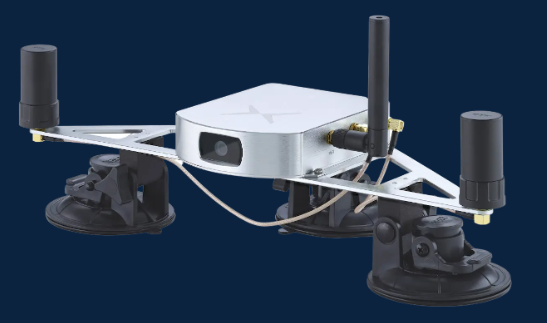
\includegraphics[width=0.75\linewidth]{img/FixpositionRTK2_Kit.png}
    \caption{Fixposition VISION-RTK 2 kit, ready-to-use view: central module with IMU, high-speed vision module, computation unit in the centre, and two GNSS antennas on the sides of the horizontal non-magnetic frame.}
    \label{fig:Fixposition RTK-2 kit}
\end{figure}


\subsubsection{Motorized zoom lens}

For our research and development, we are focusing on affordable yet scalable solutions for visual navigation systems. One critical component in our setup is a motorized zoom lens mounted on a 2-axis gimbal (pan-tilt module) \ref{fig:Pan-Tilt-Zoom_body}, which enables active software control for enhanced visual capabilities. This setup is crucial for tasks that require dynamic adjustment of the field of view and stabilization, such as autonomous navigation and precise environmental mapping \cite{PointMeIntoRightDirection}.

We are exploring industrial kits that offer a balance between performance and cost-effectiveness. The chosen model for our current application is the L085-DEVKIT from Kurokesu with a 25x zoom \cite{kurokesu_l085_devkit}, depicted at \ref{fig:kurokesu_lens}. This kit provides a robust motorized zoom lens that can be actively controlled via software, allowing for fine-tuned adjustments during operation. This flexibility makes it suitable for various platforms and applications, ensuring scalability as needed. Yet, such equipment has operational challenges, including custom calibration protocols and adaptation for image processing algorithms. However, much of this has been addressed during the first year of our project, as noted in the Early Results section.

\begin{figure}[ht]
    \centering
    \begin{subfigure}[b]{0.45\linewidth}
        \centering
        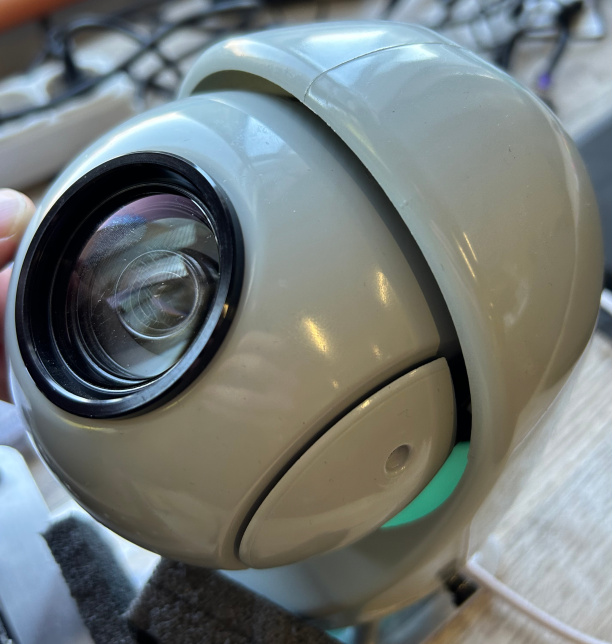
\includegraphics[width=\linewidth]{img/PanTiltZoom_camera_setup.png}
        \caption{Pan-tilt-zoom camera: appearance in assembly}
        \label{fig:Pan-Tilt-Zoom_body}
    \end{subfigure}
    \hfill
    \begin{subfigure}[b]{0.45\linewidth}
        \centering
        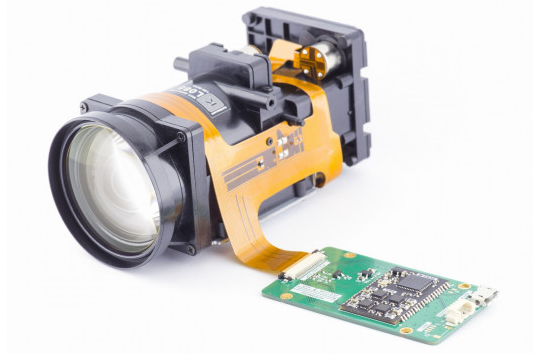
\includegraphics[width=\linewidth]{img/ZoomLense.png}
        \caption{Component view: Kurokesu L085 Zoom lens devkit}
        \label{fig:kurokesu_lens}
    \end{subfigure}
    \caption{Active Pan-tilt-zoom camera equipment}
    \label{fig:side_by_side}
\end{figure}

\textbf{Potential additional research gap:}

If we go further in focus calibration of the motorized zoom cameras, we can use them for distance measurement aid by adjusting the camera's zoom, focus, and aperture to ensure a narrow depth of field range at various distances. Precise calibration allows the system to exploit the Depth From Focus (DFF) effect, which uses the sharpness variation in images captured at different focal lengths to estimate the distance to objects.

\textbf{Opportunity with Well-Calibrated Systems:}

The measurement will only be approximate and will depend on lens properties. By adjusting the aperture, the system can create a series of images with varying sharpness, allowing it to estimate the distance to objects based on the blur gradient. There is no clarity if this approach is covered in research due to its narrow applications; Preliminary analysis of the published and patented materials shows that there is an opportunity to spot the research gap \cite{morrison_coded_apperture_2009vision}.

Benefits:
    \textbf{Graph-Based Navigation:} This method is particularly useful for graph-based visual navigation, where distinguishing between different locations is critical. The DFF effect can provide sufficient accuracy to differentiate between multiple potential paths or landmarks.
    \textbf{Enhanced Precision:} While not super-precise, this approach offers at least some degree of precision in the situations of unknown object observation: in such a case from a monocular camera, we are unable to define the size of an object and distance to it simultaneously. Thou, in this case, we inherently suffer from the optical illusion \ref{fig:scale-illusion}.
    \begin{figure}
        \centering
        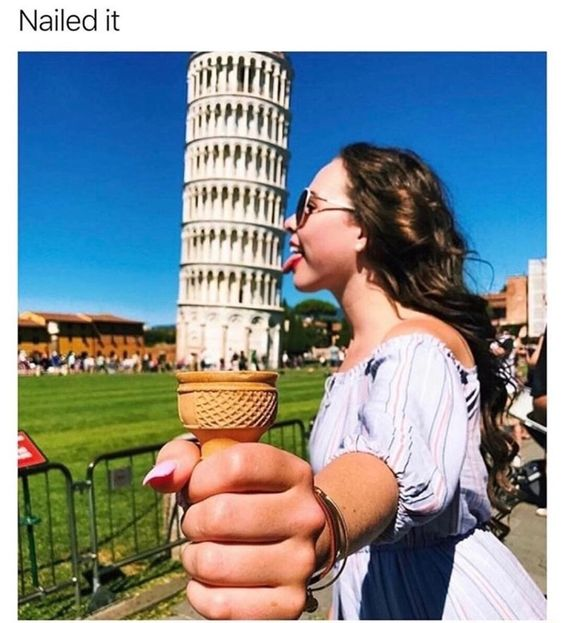
\includegraphics[width=0.5\linewidth]{img/Optical_illusion.png}
        \caption{Example of famous monocular scale ambiguity illusion}
        \label{fig:scale-illusion}
    \end{figure}

\subsubsection{LIDAR}

For our purposes, the Hokuyo UTM-30LX \cite{hokuyo_utm_30lx_ew} is an excellent choice. It offers a broad scanning range of 30 meters and performs well in outdoor conditions, providing protection from the elements \cite{RangeSensorsEvalutation}. Additionally, its wide adoption in the community enhances its value \cite{UTM_30LX_Demski2013}.

This piece of equipment will serve an assistive yet crucial role in the entire experimental pipeline. We aim to evaluate the performance of long-range navigation and localization subsystems. Fortunately, the ROS infrastructure architecture allows us to effectively separate concerns for other modules. The LIDAR will assist the course-facing RGB camera in local path planning and obstacle avoidance. This setup is a common standard in the field of outdoor UGV operations and forms the basis for several local path planning systems, such as Move Base Flex \cite{move_base_flex} and the TEB Planner \cite{TEB_Planner}. This subsystem will have fixed parameters and configuration throughout all planned experiments in this research.


\comment{WIP, we may drop this subsection}
\subsection{Datasets and Simulations}

\subsubsection{Standalone}
\paragraph{UTIAS} In our gradual development approach, we will utilize existing datasets that constitute a closed-loop series of UAV flying over the same environment, similar to the CLOUD dataset \cite{CLOUDdataset}. This dataset has selectively chosen pertinent data samples from past UAV outdoor localization studies, including the notable UTIAS dataset \cite{UTIAS}. The UTIAS dataset encompasses drone imagery across repeated flight trajectories over fields and outdoor environments in varying seasons and lighting conditions. Despite this dataset being collected with UAV flight modality, we can use the low-altitude flight recordings for our purposes of robust environment extraction evaluation.
This dataset, with its recurrent loop trajectories over the same or partially overlapping landscapes, aligns well with our research's problem setup. It allows us to gauge localization persistence while incrementally refining the topological visual landmarks map of the environment.

\paragraph{Paris-CARLA-3D}
The Paris-CARLA-3D dataset is a comprehensive resource designed for the development and testing of autonomous driving systems in urban environments. \cite{ParisCarla3D} It is derived from the CARLA simulator, a popular open-source simulator for autonomous driving research. This dataset offers detailed 3D representations of Paris-like urban landscapes. We plan to use elements from this dataset as landmarks for the training of the visual landmarks learning and detection subsystem.

\paragraph{KITTI Dataset}
The KITTI \cite{Geiger2013IJRR} dataset is one of the most widely used benchmarks for developing and evaluating autonomous driving systems. Created by the Karlsruhe Institute of Technology and the Toyota Technological Institute in Chicago, it contains many real-world traffic scenarios captured by a suite of sensors, including high-resolution RGB cameras, 3D laser scanners, and GPS/IMU systems. The dataset covers diverse driving environments such as urban, rural, and highway settings. It provides detailed annotations for a variety of tasks, including stereo vision, optical flow, visual odometry, 3D object detection, and 3D tracking. This dataset is suitable for work on map creation and self-localization precision since we have the ground truth data for all the positions in the images of the surrounding world. As well we can find the positions of the environmental elements if they are marked by the LIDAR sensor readings. Data points collected in rural environments are of special interest to us.

\subsubsection{Simulations as the development tool}
The first-phase method components could be created and tested on fixed datasets. However, the backtracking phase to the home base necessitates an open environment with decision-making opportunities. Due to dataset constraints on agent positioning space, open-world simulation becomes crucial. It notably enhances the development and testing of the "active" navigation component, enabling route formation decisions.
We intend to develop the navigating agent using the ROS system \cite{ROS2}, granting access to various simulators ranging from simpler ones like Gazebo \cite{Gazebo} to more sophisticated options such as NVIDIA's Isaac Sim.
Additionally, we can explore simulations based on high-resolution satellite imagery or images taken from drones at higher altitudes, as pursued in prior research \cite{GPS-denied-Warren} \cite{gurgu2022vision}.
Simulation provides the advantage of generating diverse scenarios for repetitive testing and designing specific corner-case experiments. This ensures that our localization system navigates effectively without getting stuck in oscillating decision situations.

\paragraph{Outdoor simulation for Husky}
To effectively evaluate the proposed navigation and localization algorithms, the interactive simulation suited for the Husky platform is much more important than the collected advanced data. There is a form of a dataset, detailed in the paper "Multi-Sensor Dataset for Benchmarking UGV Navigation in Unstructured Environments" from MDPI Sensors \cite{AutomaticallyAnnotatedOutdoorsGazebo} that contains a preconfigured set of outdoor environment simulations with different modalities available for labelling information layers, see the \ref{fig:2x2grid}.
 The most important feature of such interactive datasets is the space for the vehicle model configuration and adjustment. We are able to add the different cameras with arbitrary configurations that will be correctly simulated. It is crucial for the purposes of our research that involves a comparison of different sensor schemes: we are able to experiment with the equipment's principal scheme before sourcing the actual hardware and spending time on its configuration. Also, we will be able to develop the PTZ active exploration system in such an environment and launch it on the hardware only when it is prepared. The only issue is the accurate representation of such hardware capabilities. If for the Husky platform itself and equipment as LIDAR \cite{hokuyo_utm_30lx_ew} we have trustworthy simulation models from the manufacturer, to work with our PTZ camera, we will need to evaluate its mechatronic and optical properties in real life to transfer them into the simulation accurately.


\begin{figure}[ht]
    \centering
    \begin{subfigure}[b]{0.6\linewidth}
        \centering
        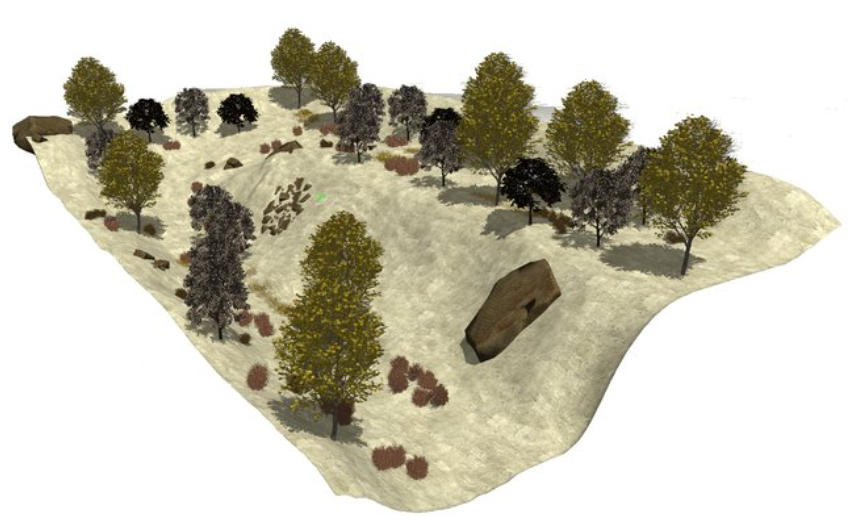
\includegraphics[width=\linewidth]{img/Rugged_Hillside_vis.png}
        \caption{Visual representation}
        \label{fig:subfig1}
    \end{subfigure}
    \hfill
    \begin{subfigure}[b]{0.3\linewidth}
        \centering
        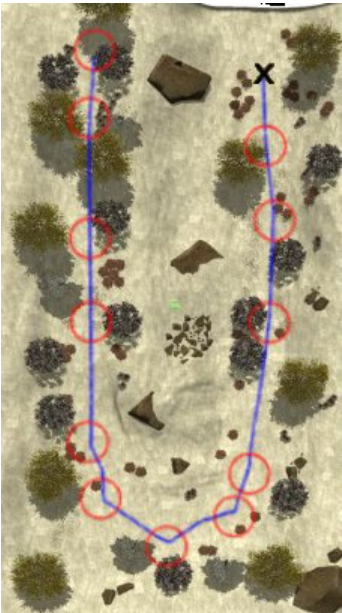
\includegraphics[width=\linewidth]{img/HillSide_PathFollowed.png}
        \caption{Path followed}
        \label{fig:subfig2}
    \end{subfigure}

    \vspace{0.3cm}

    \begin{subfigure}[b]{0.6\linewidth}
        \centering
        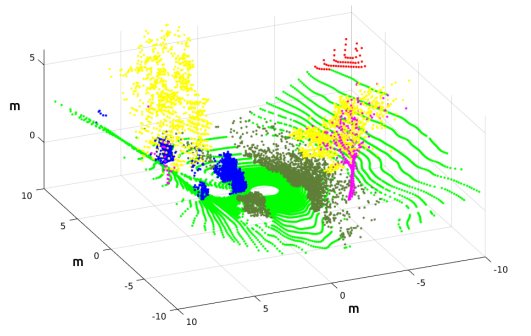
\includegraphics[width=\linewidth]{img/Hill_annotated_point_cloud.png}
        \caption{Annotated point cloud}
        \label{fig:subfig3}
    \end{subfigure}
    \hfill
    \begin{subfigure}[b]{0.3\linewidth}
        \centering
        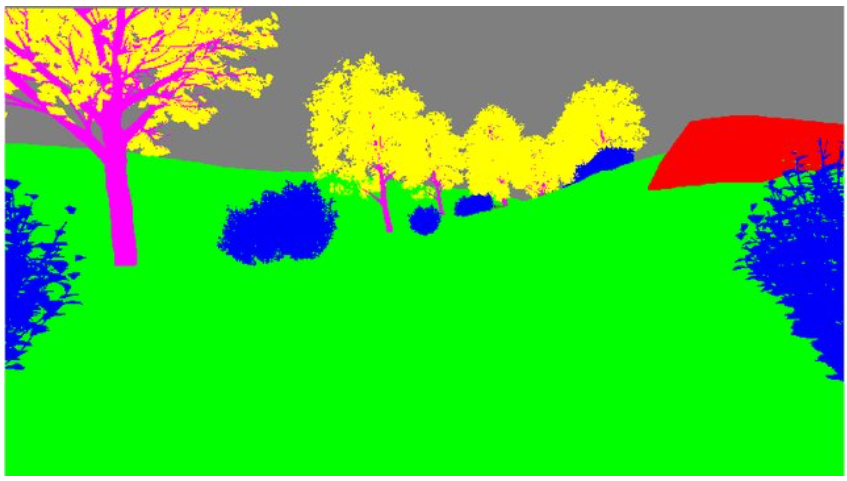
\includegraphics[width=\linewidth]{img/FirstPerson_Annotated_Hillside.png}
        \caption{Annotated onboard camera view}
        \label{fig:subfig4}
    \end{subfigure}

    \caption{Different views of the same simulated environment in Gazebo sim}
    \label{fig:2x2grid}
\end{figure}


 \todo{Write about photorealistic simulations for the visual algorithms evaluation}


\comment{Fine to read, minor todos}

\section{Early Results }
% \todo{In this section, our initial results are presented.
% What has been done in Y1?
% What part of your background will be covered by these results?
% }

% \begin{itemize}
\paragraph{Research in adjacent to Visual Odometry field:}
    The current state-of-the-art in robust parameter fitting algorithms has been thoroughly investigated, with a focus on recent advancements in robust parameter estimation methods, such as MAGSAC++ \cite{burgard1997active}. This line of research is in progress, and intermediate findings are being developed into a comprehensive study, which should culminate in a publishable paper.
    With an operational platform and navigation solution, we can evaluate the performance of those algorithms for visual localization problems and open the avenue for further development of tailored solutions for our setup.

\paragraph{Topic Clarification:}
    Compared to the initial research focus, the topic has been revised to align with the current developments, state of research, and emerging problems in Ukraine. This adjustment reflects the rapidly evolving situation and the realistic pace of academic research achievable by our working group.

\paragraph{Sourcing Platforms and Industrial Partnerships:}
    Although this aspect is primarily technical, it has significantly impacted our project. We have successfully sourced the necessary hardware platforms and established valuable industrial partnerships supporting our research objectives. The hardware workshop for support of these platforms is fully operational and reliable.

\paragraph{Pan-Tilt-Zoom visuomotor system calibration:}
    Over the past year, we have completed several successful R\&D projects using our target sensing platform. This includes camera calibration and the development of dedicated image processing approaches. Currently, members of the robotics laboratory are working on accurate control and positioning of the pan-tilt platform itself. This expertise, combined with access to industrial resources for support and integration, gives us confidence in the success of the vision control component and the pace of related experiments.



\comment{Fine to read}

\section{Conclusive Remarks}
% \todo[inline]{
%     \begin{itemize}
%         \item What is proposed? Is it methodologically mature and sound? – Why? (Done?)
%         \item What is the envisioned contribution? (Done)
%         \item What are the early results? (...)
%         \item What are envisioned use cases and their estimated impact? (Done)
%         \item What is the planned short-/medium-/long-term future work? (planned)
%     \end{itemize}


This PhD proposal outlines a comprehensive research plan to advance the field of autonomous navigation and mapping in unstructured outdoor environments. Our primary focus is on leveraging the capabilities of pan-tilt-zoom (PTZ) cameras to enhance the reliability and efficiency of Unmanned Ground Vehicles (UGVs) in complex, real-world settings to make the UGV's autonomous recovery more reliable in unstructured outdoor environments.

Our review of the current state-of-the-art has highlighted several critical gaps and challenges that our research intends to address, with a particular emphasis on the innovative application of PTZ cameras:

\begin{itemize}
\item \textbf{Enhanced Visual Perception:} The PTZ camera's ability to dynamically adjust its field of view allows for more effective visual feature extraction and image matching, even in dynamic and unstructured environments. Our research will explore how PTZ cameras can improve the detection and recognition of visual landmarks by providing multiple perspectives and focusing on relevant features.
\item \textbf{Improved Topological Mapping:} By integrating PTZ cameras, we can create more detailed and adaptable topological maps. These maps will benefit from the PTZ camera's ability to zoom in on critical areas and capture high-resolution images, facilitating better place recognition and reducing the ambiguity often associated with large, unstructured environments.
\item \textbf{Advanced Landmark-Based Localization:} The PTZ camera's capability to actively track and focus on visual landmarks will enhance the accuracy and robustness of localization. This will be particularly valuable in environments where traditional GPS-based methods are unreliable. Our research will develop techniques to optimize the use of PTZ cameras for continuous and dependable landmark detection.
\item \textbf{Seamless System Integration:} The dynamic control of PTZ cameras will be integrated into our mapping and navigation systems, addressing practical challenges such as battery life constraints and real-time operation in dynamic environments. This integration aims to create a cohesive system that leverages the PTZ camera's flexibility for improved navigation performance.
\end{itemize}

Understanding the special features of unstructured outdoor environments—such as irregular terrain, dynamic elements, sparse visual landmarks, varied vegetation, and changing weather conditions—is crucial for developing robust systems. The PTZ camera's adaptability suits these challenges, allowing for real-time adjustments and focused data collection.

% \todo[inline]{Specify timeline (Once the Methodology will be covered)
% \begin{itemize}
%     \item \textbf{Short-term:} Platform components integration, Q4 and Q1.
%     \item \textbf{Mid-term:} Recovering via backtracking. Research of the optimal conditions for Q1, Q2.
%     \item \textbf{Long-term:} Q3, Patrolling.
%     \item \textbf{Future:} Movement towards autonomous operations that include exploration of unseen environments.
% \end{itemize}
% }

The expected \textbf{contributions} of this research include:

\begin{itemize}
\item The development of novel visual perception algorithms optimized for PTZ cameras in unstructured environments.
\item A hybrid topological-metric mapping framework that benefits from the PTZ camera's enhanced visual data.
\item Advanced landmark-based localization techniques utilizing the PTZ camera's dynamic tracking capabilities.
\item Integrated systems that combine the PTZ camera's strengths with mapping and navigation processes to operate efficiently in real-time and under practical constraints.
\end{itemize}

Ultimately, this research aims to significantly improve the capabilities of autonomous UGVs, enabling them to navigate complex and dynamic outdoor environments with greater accuracy and reliability. The innovative use of PTZ cameras will not only contribute to the academic understanding of autonomous systems but also have practical implications for various applications, including environmental monitoring, search and rescue operations, and agricultural automation. The

By focusing on the unique advantages of PTZ cameras, this research will push the boundaries of current technology, providing new insights and solutions extending outdoor autonomous navigation capabilities. Integrating PTZ cameras into our proposed system configuration promises to enhance real-world efficiency and reliability, making a meaningful impact on both scientific research and practical applications.



% Please note that the first paragraph of a section or subsection is
% not indented. The first paragraph that follows a table, figure,
% equation etc. does not need an indent, either.


% Subsequent paragraphs, however, are indented.

% \subsubsection{Sample Heading (Third Level)} Only two levels of
% headings should be numbered. Lower level headings remain unnumbered;
% they are formatted as run-in headings.

% \paragraph{Sample Heading (Fourth Level)}
% The contribution should contain no more than four levels of
% headings. Table~\ref{tab1} gives a summary of all heading levels.

%
% the environments 'definition', 'lemma', 'proposition', 'corollary',
% 'remark', and 'example' are defined in the LLNCS documentclass as well.
%

\printbibliography


\end{document}
```
